\documentclass[
	aspectratio=169,	% Modern aspect ratio (TODO: Other ratios not yet supported)
	onlytextwidth,		% Sets totalwidth=\textwidth and therefore e.g. columns won't invade the margins
	t,					% Default vertical alignment of frames and colums at top (default is centered) % Stored in \beamer@centered (\beamer@centeredfalse, \beamer@centeredtrue)
%	handout,			% Create a basic handout of the presentation (removes overlays)
	]{beamer}

%%%%%%%%%%%%%%%%%%%%%%%%%%%%%%%%%%%%%%%%%%
% 1) Load the desired presentation theme
\usetheme[
% Individual options to customize the presentation conforming to the corporate design
	hs,					% Change default faculty color set and predefined faculty values: hs or <empty> (default), inw, cb, me, sw, wi, inst (\renewcommand{\insertfacultyname}{Institutname} needed)
	language=english,	% Change language to english (default: ngerman), other languages are possible (see babel-package) but may need further adjustments 
	toc,				% Adds a ToC slide
	sectionslide,		% Display separate section slides
	subsectionslide,		% Display separate subsection slides containing section and subsection name
%	smallpagenumber,	% Reduces the size of the page number
%	nototalpages,		% Hides the total number of slide in footline
%	nofacultyicon,		% Hides the faculty icon on title page
	colormath=nottext,	% Enables coloring of math text: off or <empty>, full, nottext (default)
%	printhandout,		% Places two slides on a single a4 paper for printing the presentation (beamer class option 'handout' needed)
%	noframesubtitle,	% Disables frame subtitles alltogether and slightly increases frame height
% Additional style options not completely conforming to the corporate design
	titlepagedate,		% Shows the date on the titelpage
	fancystyle,			% Enables some fancy styles, that are not part of the corporate design specifications (default: off)
%	progressbar,		% Shows the progressbar in footline (run twice to update progressbar)
	]{hsmw} 

%%%%%%%%%%%%%%%%%%%%%%%%%%%%%%%%%%%%%%%%%%
% 2) Specify default fields for presentation and pdf document properties
% Set the title: \title{Long title everywhere} or \title[Short title for footline]{Long title for titlepage}
\title[Cognitive Science and Machine Learning]{Cognitive Science and Machine Learning}
\subtitle{}
% Authors (separate multiple author names e.g. with \and for additional space): \author{author for everywhere} or \author[author for footline]{author for titlepage and thankyouslide}
\author[Mert Saruhan]{Mert Saruhan, B.Sc.}
% Institute (will be prefilled automatically, depending on chosen faculty theme option): \institute{institute for everywhere} or \institute[institute for footline and thankyouslide]{institute for titlepage}
%\institute[Fakultät Angewandte Computer und Biowissenschaften]{Fakultät Angewandte Computer und Biowissenschaften}
% Date of presentation (\today or a fixed value): \date{date for everywhere} or \date[date for footline]{date for titlepage}
\date{\today} % 22. März 2022
% Impressum for thankyou slide (leave one empty if not wanted or needed):
\email{msaruhan@hs-mittweida.de} % \email{E-Mail}
\courseofstudies{Mathematics for Network and Data Science (MA20w1-M)} % \courseofstudies{Course of Studies (Group Number)}
%\additional[Sidebar Text]{Main Text} % Additional information you may want to give (Department, Module, etc.) \additional[Sidebar Text]{Main Text}

%%%%%%%%%%%%%%%%%%%%%%%%%%%%%%%%%%%%%%%%%%
% 3) Use features
% Titlegraphic changes the title page to "wide" (default) if left empty or inserts given image (by file path) and scales to 6.2cm height otherwise:
\titlegraphic{} %\titlegraphic{figures/thankyou.jpg}

%%%%%%%%%%%%%%%%%%%%%%%%%%%%%%%%%%%%%%%%%%
% 4) Add bibliography
% Load the package and options you like, e.g. for recommended ieee style in combination of biblatex and biber:
\usepackage[backend=biber, bibstyle=ieee, citestyle=numeric-comp, sorting=none, natbib=true, hyperref=true, dashed=false]{biblatex}
% Add your bibliography file(s)
\addbibresource{ref.bib} 
% Dont forget to use \makebibliography where you want to put it, e.g. at the end of your presentation, after the "normal" slides:
% \appendix
% \makebibliography
% Compile with following command sequence to fully include bibliography: pdflatex, biber, pdflatex, pdflatex

%%%%%%%%%%%%%%%%%%%%%%%%%%%%%%%%%%%%%%%%%%
% 5) Existing macro usage examples

% \appendix is used as end marker for slides (slide numbers and progressbar)
% \makethankyou creates a thank you slide and is used as end marker for slides (progressbar)
% \makebibliography creates one or multiple bibliography slides

% For multiple speakers you can use \setcurrentspeaker{speaker name} or \setcurrentspeaker*{speaker name} prior to the frame
% To reset to the default author, use \resetcurrentspeaker{} or \resetcurrentspeaker*{}
% Starred versions of these macros prepend the word "speaker"

%%%%%%%%%%%%%%%%%%%%%%%%%%%%%%%%%%%%%%%%%%
% 6) Import additional packages you need, (re-)define macros and create a wonderful latex presentation
\usepackage{tikz}
\usetikzlibrary{arrows.meta}
\setbeamertemplate{caption}{\insertcaption}
\usepackage{xcolor}
% You can remove this package - it is only needed for the dummy content
\usepackage{blindtext}

%%%%%%%%%%%%%%%%%%%%%%%%%%%%%%%%%%%%%%%%%%
\begin{document}

	\section{What is Cognitive Bias?}
	
	\begin{frame}[fragile]{What is Cognitive Bias?}{Introduction}
		
		
		\begin{enumerate} 
			\item<1-> Bias created by human cognition
			\item<2-> Has an active role in decision making 
			\item<3-> Not always logical
			\item<4-> Notation: $ B(q|p) $,
			How strongly one belives q occurs after observing p
			\item <5-> $ 0 \leq B(q|p) \leq 1 $
		\end{enumerate}

	\begin{frame}[fragile]{What is Cognitive Bias?}{Types of cognitive bias we use}
		
		\begin{itemize}	
			
			\item<1-> \textbf{Symmetry Bias} \newline
			\textbf{Example}: `If the weather was rainy, then the ground is wet' \newline
			\uncover<2->{$\implies$ `Only if the ground is wet, then the weather was rainy a while ago'~\cite{shi07}}
			\item<3-> \textbf{Mutual Exclusitivity Bias} \newline
			\textbf{Example}: `if you do not clean your room, then you will not be allowed to play' \newline
			\uncover<4->{$\implies$ `if I clean up my room, then my mom will allow me to play'~\cite{hat07}}
		
		\end{itemize}
	
	\end{frame}
	
	\begin{frame}[fragile]{What is Cognitive Bias?}{Illogical bias}
		
		$p$: `The shoe is white' \newline
		$q$: `A star is printed on it' \newline
		\uncover<2->{$p\implies q$: `If the shoe is white, then a star is printed on it'~\cite{tan18}} \newline

		\uncover<3->{\textbf{Symmetry Bias} \newline
		$q \implies p$: `If a star is printed on a shoe, then the shoe is white'~\cite{tan18}} \newline

		\uncover<4->{\textbf{Mutual Exclusitivity Bias} \newline
		$\neg p \implies \neg q$: `If the shoe is not white, then a star is not printed on it'~\cite{tan18}} \newline

	\end{frame}

	\begin{frame}[fragile]{What is Cognitive Bias?}{Properties and biases}
		\vfill
	
		\begin{itemize}	
			
			\item<1-> \textbf{Symmetry Bias (S)}: \hfill $B(q|p) \sim B(p|q)$ 
			\item<2-> \textbf{Mutual Exclusitivity Bias (MX)}: \hfill $B(q|p) \sim B(\neg q| \neg p)$ 
			\item<3-> \textbf{The law of excluded middle (XM)}: \hfill $B(q|p) \sim 1- B(\neg q|p)$ 
			\item<4-> \textbf{Estimation relativity (ER)}: \hfill $B(q|p) \sim 1- B(q|\neg p)$ 
		
		\end{itemize}
	
		\vfill
		Note: Adapted from~\cite{tak10}
	\end{frame}

	\section{ML Implementation}

	\begin{frame}[fragile]{ML Implementation}{Interpretation}
		\begin{columns}

			\begin{column}[T]{.25\textwidth}
				\begin{table}
					
					\begin{tabular}{|c|c|c|}
						\hline
						& \textbf{$q$} & \textbf{$\neg q$} \\
						\hline
						\textbf{$p$} & a & b \\
						\hline
						\textbf{$\neg p$} & c & d \\
						\hline
					\end{tabular}
					\caption{Co-occurence frequency~\cite{man21}}
				
				\end{table}
			\end{column}

			\begin{column}[T]{.15\textwidth}
				\uncover<3->{
					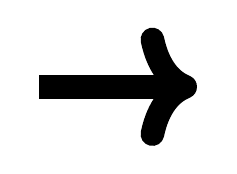
\begin{tikzpicture}
						\draw[->, line width=3mm] (8,-9) -- (10,-9);
						\end{tikzpicture}
				}
			\end{column}

			\begin{column}[T]{.59\textwidth}
				\uncover<3->{
					\begin{table}
						\begin{tabular}{|c|c|c|}
							\hline
							& \textbf{$L(x) = L(w^{x})$} & \textbf{$L(x) \neq L(w^{x})$} \\
							\hline
							\textbf{$L(w_{i}) = L(w^{x})$} & a & b \\
							\hline
							\textbf{$L(w_{i}) \neq L(w^{x})$} & c & d \\
							\hline
						\end{tabular}
						\caption{ML implementation of the co-occurence frequency table~\cite{man21}}
					
					\end{table}
				}
				
				\uncover<2->{\begin{itemize}
					\item $x$: sample
					\item $w_{i}$: $i^{\text{th}}$ prototype
					\item $w_{x}$: winner prototype of sample x
					\item $L(y)$: label of y
				\end{itemize}}
			\end{column}

		\end{columns}
	\end{frame}
		
	\begin{frame}[fragile]{ML Implementation}{Updating learning rates}
	
		\centering
				\includegraphics[width=.4\textwidth]{myfigs/lr flowchart1.png}
				\captionof{figure}{Learning rate update flowchart part 1~\cite{tak10}}
	\end{frame}

	\begin{frame}[fragile]{ML Implementation}{Updating learning rates}
	
		\centering
				\includegraphics[width=.4\textwidth]{myfigs/lr flowchart2.png}
				\captionof{figure}{Learning rate update flowchart part 2~\cite{tak10}}
	\end{frame}

	\begin{frame}{ML Implementation}{Updating learning rates}
		\vfill
		\begin{itemize}
			\item<1->$R_{i}(a_{i},b_{i},c_{i},d_{i},t)$: Causal relationship between events for $i^{\text{th}}$ prototype at time $t$
			\item<2->$\epsilon_{i}(t) = 1- R_{i}(t)$: Local learning rate of $i^{\text{th}}$ prototype at time $t$
			\item <3-> Each prototype share learning rate with their class!
		\end{itemize}
		\vfill

	\end{frame}


	\section{Optimizers}
	
	\begin{frame}[fragile]{Optimizers}{Loose Symmetry (LS)}

		\begin{itemize}
			
		\item<1-> $R^{\text{LS}}_{i}(t) = \frac{a_{i}(t) 
		+ \frac{b_{i}(t)}{b_{i}(t) + d_{i}(t)}d_{i}(t)}
		{a_{i}(t) 
		+ \frac{b_{i}(t)}{b_{i}(t) + d_{i}(t)}d_{i}(t) 
		+ b_{i}(t) 
		+ \frac{a_{i}(t)}{a_{i}(t) + c_{i}(t)}c_{i}(t)}$~\cite{tak10, man21} 
		\vspace{10pt}
		\item<2-> Satisfies XM and loosely satisfies S, MX, and ER~\cite{tak10} 
		\item <3-> Has better results than other cognitive bias optimizers in tested datasets~\cite{tak10} 
		\end{itemize}
	\end{frame}

	\begin{frame}[fragile]{Optimizers}{Loose Symmetry under Rarity (LSR)}

		\begin{itemize}

		\item<1-> Assumption: The events $p$ and $q$ are small, hence the correlation of any two events is unlikely, $d(t) \rightarrow \infty$~\cite{hat07}
		\item <2-> Example: The correlation between any random event and you starting you car in the morning~\cite{hat07}
		\item<3-> $R^{\text{LSR}}_{i}(t) = \lim_{d_{i}(t) \to \infty}R^{\text{LS}}_{i}(t)$
		\vspace{10pt}
		\item<4-> $R^{\text{LSR}}_{i}(t) = \frac{a_{i}(t) 
		+ b_{i}(t)}
		{a_{i}(t) 
		+ 2b_{i}(t) 
		+ \frac{a_{i}(t)}{a_{i}(t) + c_{i}(t)}c_{i}(t)}$~\cite{tak10}
		\vspace{10pt}
		\item<5-> Satisfies S~\cite{tak10}
		\end{itemize}
	\end{frame}
	\section{Results}

	\begin{frame}[T]{Results}

		\begin{itemize}

		\item<1-> Compare the performance cognitive models with OGVLQ model
		\item<2-> OGLVQ model stands for optimized GLVQ~\cite{OGLVQ}
		\item<3-> For balanced dataset, use accuracy as score
		\item<4-> For Imbalanced dataset, use F1 score as score
		\end{itemize}
	\end{frame}
	
	\begin{frame}[fragile]{Results}{Balanced dataset}
		\scriptsize
		Dataset: Ionosphere dataset~\cite{ion} 
		\newline
		
		\begin{columns}
			
			\begin{column}[T]{0.33\textwidth}
				\begin{figure}
					\includegraphics[width=0.9\textwidth]{myfigs/LS_b.png}
				\end{figure}
			\end{column}
		
			\begin{column}[T]{0.33\textwidth}
				\begin{figure}
					\includegraphics[width=0.9\textwidth]{myfigs/LSR_b.png}
				\end{figure}
			\end{column}
		
			\begin{column}[T]{0.33\textwidth}
				\begin{figure}
					\includegraphics[width=0.9\textwidth]{myfigs/OGLVQ_b.png}
				\end{figure}
			\end{column}
		
			
		\end{columns}
		
		\centering		\color{red}{Be careful with y-axis, since they do not share common size}
	
	\end{frame}
	
	\begin{frame}[fragile]{Results}{Balanced dataset}
		\scriptsize
		Dataset: Ionosphere dataset~\cite{ion} 
		\newline
		\begin{columns}
			
				\begin{column}[T]{0.33\textwidth}
						\begin{figure}
					\includegraphics[width=0.9\textwidth]{myfigs/LS_b_res.png}
				\end{figure}
			\end{column}
		
			\begin{column}[T]{0.33\textwidth}
					\begin{figure}
					\includegraphics[width=0.9\textwidth]{myfigs/LSR_b_res.png}
				\end{figure}
			\end{column}
		
			\begin{column}[T]{0.33\textwidth}
				\begin{figure}
						\includegraphics[width=0.9\textwidth]{myfigs/OGLVQ_b_res.png}
					\end{figure}
				\end{column}
			
			
			\end{columns}
			
		\end{frame}
		
		\begin{frame}[fragile]{Results}{Imbalanced dataset}
			\scriptsize
			Dataset: Ionosphere dataset~\cite{ion} 
			\newline
			
			\begin{columns}
				
			\begin{column}[T]{0.33\textwidth}
				\begin{figure}
					\includegraphics[width=0.9\textwidth]{myfigs/LS_i.png}
				\end{figure}
			\end{column}
			
			\begin{column}[T]{0.33\textwidth}
				\begin{figure}
					\includegraphics[width=0.9\textwidth]{myfigs/LSR_i.png}
				\end{figure}
			\end{column}
			
			\begin{column}[T]{0.33\textwidth}
				\begin{figure}
					\includegraphics[width=0.9\textwidth]{myfigs/OGLVQ_i.png}
				\end{figure}
			\end{column}
			
			
		\end{columns}
		
		\centering		\color{red}{Be careful with y-axis, since they do not share common size}
		
	\end{frame}
	
	\begin{frame}[fragile]{Results}{Imbalanced dataset} 
		\scriptsize
		Dataset: Ionosphere dataset~\cite{ion} 
		\newline
		\begin{columns}
			
			\begin{column}[T]{0.33\textwidth}
				\begin{figure}
					\includegraphics[width=0.9\textwidth]{myfigs/LS_i_res.png}
				\end{figure}
			\end{column}
		
			\begin{column}[T]{0.33\textwidth}
				\begin{figure}
					\includegraphics[width=0.9\textwidth]{myfigs/LSR_i_res.png}
				\end{figure}
			\end{column}
		
			\begin{column}[T]{0.33\textwidth}
				\begin{figure}
					\includegraphics[width=0.9\textwidth]{myfigs/OGLVQ_i_res.png}
				\end{figure}
			\end{column}
		
			
		\end{columns}
		
	
	\end{frame}
	
	
	\begin{frame}{fragile}{Conclusion}
		
		Cognitive bias optimizer ...
		\begin{itemize}
			\item <1-> use same learning rate for each prototype in the same class
			\item <2-> have better learning rate graphs than OGLVQ
			\item <3->  have better learning performance than OGLVQ

		\end{itemize}
		
	\end{frame}

	\begin{frame}{fragile}{Further}
	
		Need further testing on
		\begin{itemize}

			\item <1-> optimized datasets
			\item <2-> noiser datasets

		\end{itemize}


	\end{frame}

	
	\appendix
	
	\makebibliography

	\makethankyou

\end{document}
